\section{Interface graphique}

\label{cli}

\subsection*{Problématique}

Après avoir travaillé sur le fonctionnement général du jeu, il est intéressant de développer une nouvelle manière de visualiser une partie. On veut notamment pouvoir naviguer entre les tours, avoir un maximum d'information sur la partie, le tout dans une interface plaisante. On s'impose également de développer cette interface en C standard.

\subsection{Stratégie}

Grâce à la structure de partie (cf \ref{game}), on a accès à l'ensemble des tours d'une partie donnée. On a donc besoin de savoir afficher un tour en entier. Pour cela on scinde l'écran en plusieurs parties.

\begin{figure}[H]
    \centering
    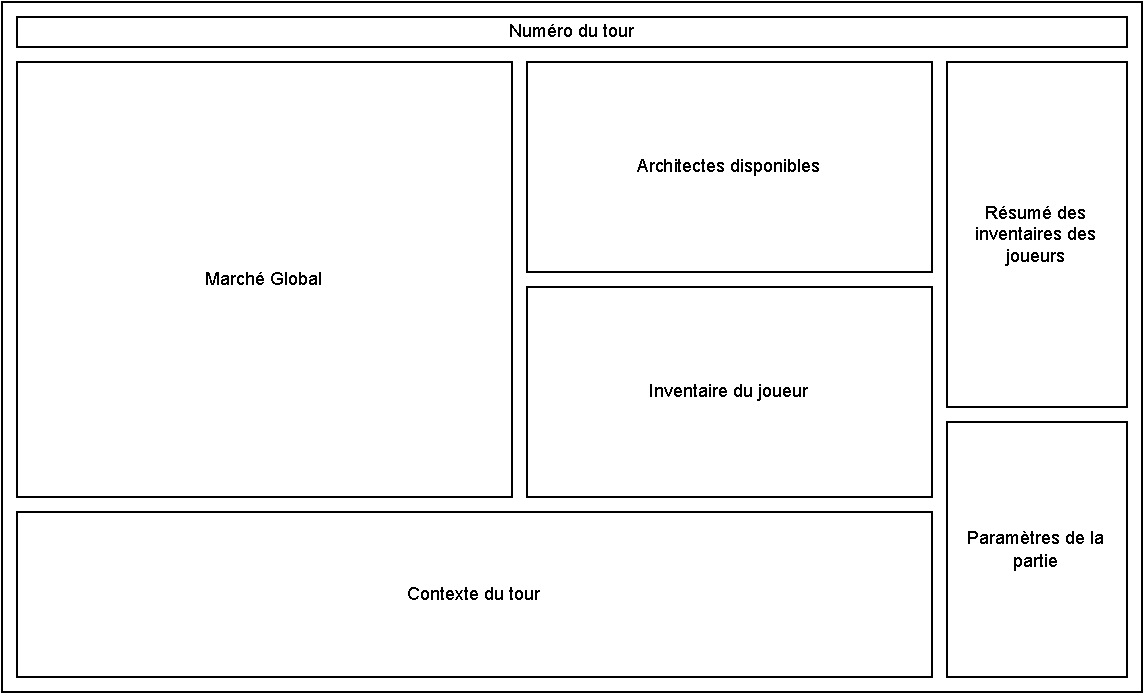
\includegraphics[width=\textwidth]{img/cli_schema.pdf}
    \caption{Schéma de l'interface}
    \label{fig:cli_schem}
\end{figure}

\subsection{Mise en oeuvre}
A l'aide de la fonction \code{print\_to\_coordinates} on est capable d'écrire aux coordonnées (x,y) le texte que l'on souhaite.

Par la suite, on doit réécrire toutes les fonctions d'affichage afin de pouvoir afficher les composants aux coordonnées souhaitées. On réutilise la même arborescence du code que pour le code principal.   

Comme pour l'évaluation de partie (cf \ref{evaluator}) et les tests (cf \ref{tests}), on créer un nouvel exécutable \code{cli}. On récupère l'entrée de l'utilisateur à l'aide de \code{getchar} et on navigue dans les tours de la partie.

\begin{lstlisting}[frame=single, caption={Navigation dans les tours de la partie}]
while (ch != 'q')
{
    switch (ch)
    {
        /* get the right turn to display */
    } 
    
    /* display the turn */
    cli_turn_display(turn);

    ch = getch();
}
\end{lstlisting}